\documentclass{article}
\usepackage[utf8]{inputenc}
\usepackage{amsmath}
\usepackage{amssymb}
\usepackage{graphicx}


\begin{document}
\section*{Complex roots}
Given a complex number $w = u +iv$ for $u,v \in \mathbb{R}$ with $v \geq 0$,its root $\sqrt{w} = x + iy$ can be defined by
\begin{align*}
    x &:= \sqrt{\frac{\sqrt{u^{2}+v^{2}} + u}{2}} \\[2mm]
    y &:= \sqrt{\frac{\sqrt{u^{2}+v^{2}} - u}{2}}
\end{align*}
\subsection*{1-11.a}
We are tasked with finding a $w = u + iv$ for which the direct implementation, i.e. using the above formulae, is prone to cancellation. We observe that the term to compute $y$ contains a difference, where if $u \gg v$ we have $\sqrt{u^{2}+v^{2}} \approx \sqrt{u^{2}} = u$ and we hence compute the difference of two almost equal numbers, hence this will cause cancellation to occur. However we can also have the case where $u < 0$, as the above case implicitly assumes that $u > 0$, and then we have that for $|u| \gg |v|$ that $\sqrt{u^{2} + v^{2}} \approx \sqrt{u^{2}} = -u$. In both cases we get that $|u| \gg |v|$ is when cancellation can occur.
\subsection*{1-11.b}
We are tasked with computing $xy$ as an expression of $u$ and $v$. We get
\begin{align*}
    xy &= \sqrt{\frac{\sqrt{u^{2}+v^{2}} + u}{2}} \cdot\sqrt{\frac{\sqrt{u^{2}+v^{2}} - u}{2}} \\
    &= \sqrt{\frac{\sqrt{u^{2}+v^{2}} + u}{2}\cdot \frac{\sqrt{u^{2}+v^{2}} - u}{2}} \\
    &= \sqrt{\frac{\left(u^{2}+v^{2}\right) -u\sqrt{u^{2} +v^{2}} + u\sqrt{u^{2}+v^{2}}- u^{2}}{4}} \\
    &= \sqrt{\frac{u^{2}+v^{2}-u^{2}}{4}} \\
    &= \sqrt{\frac{v^{2}}{4}} \\
    &= \frac{v}{2}
\end{align*}

\pagebreak

\subsection*{1-11.c}
We are tasked with implementing an implementation that is not vulnerable to cancellation. We use the result from 11-1.b and the insights gained in 1-11.a to see that only one of the formulae can be prone to cancellation. For $u > 0$ the formula for $y$ is prone to cancellation and for $u < 0$ the formula for $x$ is prone to cancellation. Hence we can always safely compute one of the formulae. We can then use that $xy = \frac{v}{2}$ which allows us to compute the other one. We hence get a modified but equivalent set of formulae
\begin{align*}
    x &=
    \begin{cases}
    \sqrt{\frac{\sqrt{u^{2}+v^{2}} + u}{2}} \quad &\text{if } u \geq 0 \\
    \qquad\:\frac{v}{2y} &\text{else}
    \end{cases} \\[2mm]
    y &=
    \begin{cases}
    \sqrt{\frac{\sqrt{u^{2}+v^{2}} - u}{2}} \quad &\text{if } u < 0 \\
    \qquad\:\frac{v}{2x} &\text{else}
    \end{cases}
\end{align*}
We can now also see that in the case that $u = 0$ we just have a real number and we can use the conventional square root, the only problem is that this does not work if the number is negative, hence we will just use the formulae above. We then implement this in code which gives us
\begin{figure}[!hbt]
    \centering
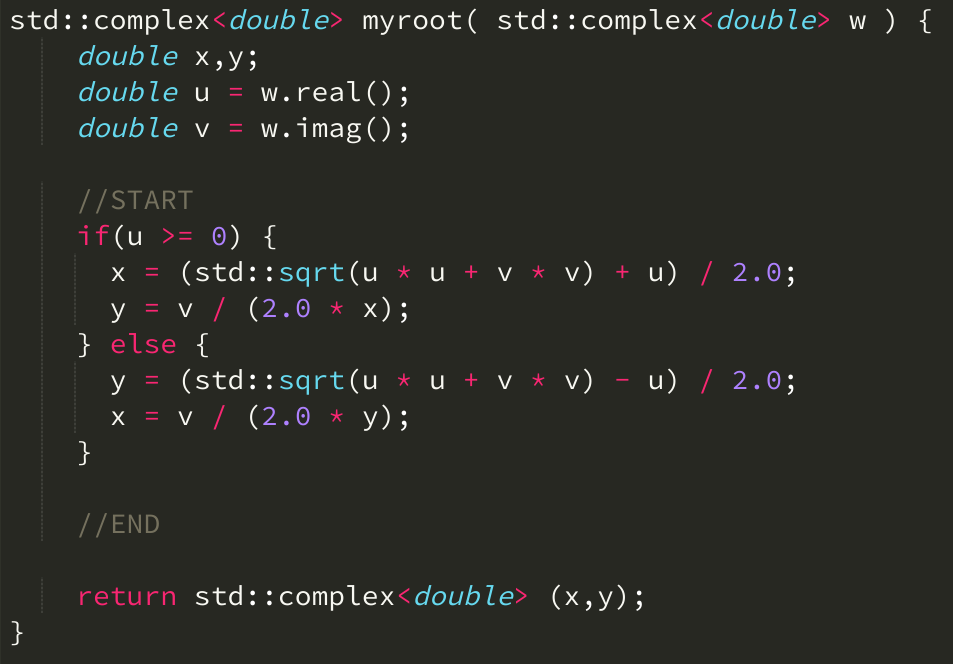
\includegraphics[width=1.0\linewidth]{1-11.c.png}
\end{figure}

\end{document}
